\subsection{Teilnahme und Login}

Beim ersten Laden der Anwendung soll eine Startseite aufgebaut werden, wie sie in Abbildung~\vref{fig:MockSignin} zu sehen ist.
Hierbei sollen Nutzer einfach an einer Umfrage teilnehmen und sich anmelden oder ein Registrierungsvorgang starten können.
Für die Teilnahme an einer Umfrage müssen die Studierenden lediglich einen \emph{Surveycode} wie \zb \texttt{W3VFG5NHY} eingeben.
Eine Anmeldung ist nicht erforderlich, um die Anonymität gemäß Anforderung~\hyperref[Anf:A14]{A14} zu wahren.
Anschließend wird der Benutzer auf die Umfrageseite weitergeleitet, auf der er die benötigten Felder ausfüllt (siehe Kapitel~\ref{ssec:konzept:client:umfrage}).
Beim Beantworten von Umfragen ist davon auszugehen, dass dies zu einem großen Teil von mobilen Endgeräten erfolgt (siehe Anforderung~\hyperref[Anf:A1]{A1}).
Diese Seiten müssen daher für die mobile Nutzung optimiert werden, dies ist jedoch nicht als Teil der Mock-Ups dargestellt.
Für angemeldete Benutzer, die Umfragen erstellen und verwalten, ist jedoch die mobile Nutzung unwahrscheinlich, da etwa Dozenten in der Regel die Vorlesungsvorbereitung an einem Desktop-Computer durchführen.
% Hierbei soll der späteren Implementierung dieser Seite der Aspekt der mobilen Benutzung beachtet werden, da viele Benutzer eine Umfrage auf ihren mobilen Endgeräten durchführen.
% Bei allen anderen Seiten soll dieser Aspekt jedoch zunächst vernachlässigt werden.

\begin{figure}[H]
	\centering
	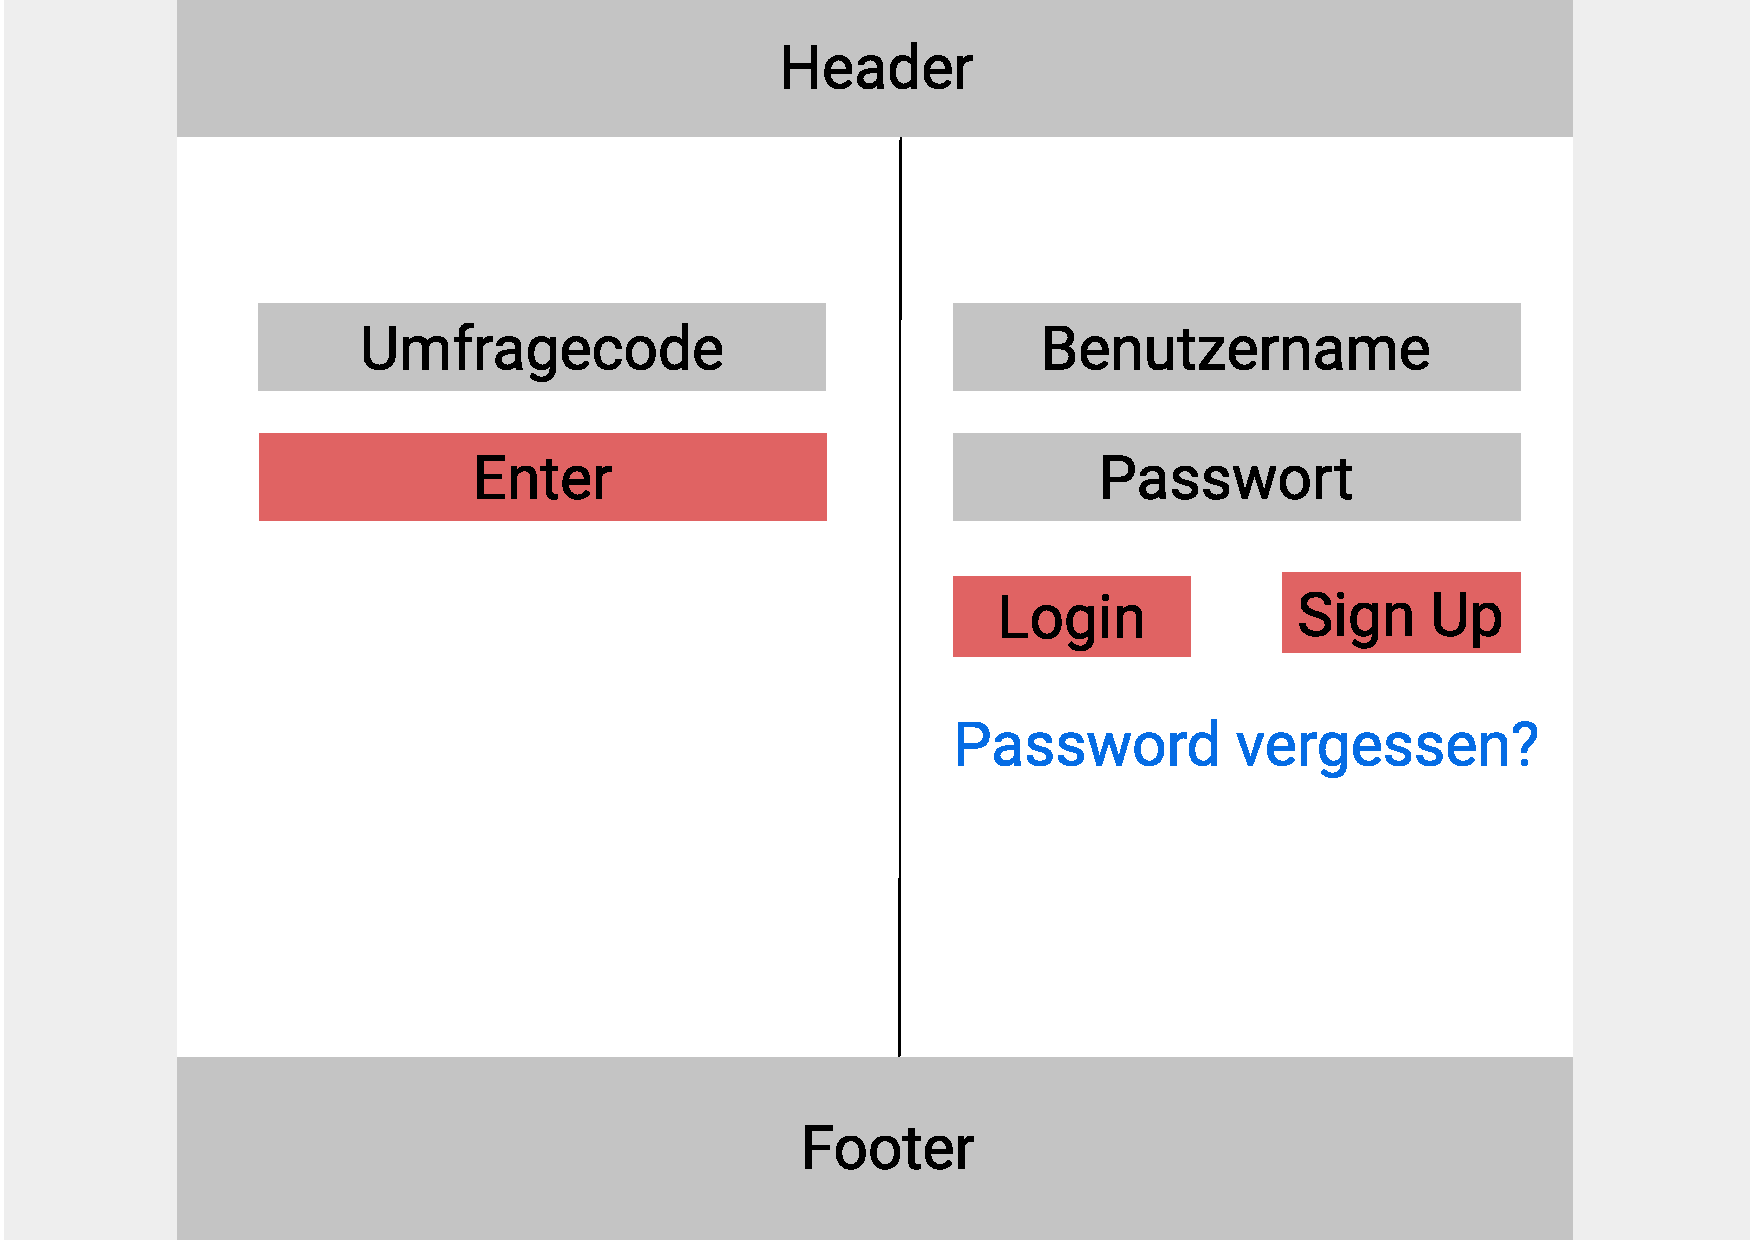
\includegraphics[width=0.7\textwidth]{img/konzeption/client/signin}
	\captionsetup{justification=centering, format=plain}
	\caption[Mock-Up der Startseite]{Mock-Up der Startseite \\\figma}
	\label{fig:MockSignin}
\end{figure}

Nutzer erhalten, wie in Abbildung~\ref{fig:MockSignin} auf der rechten Seiten sichtbar, ebenfalls die bereits angesprochene Anmelde-Möglichkeit.
Hierzu soll der \emph{Benutzername} und das \emph{Passwort} eines existierenden Benutzers eingegeben werden.
Nach einer erfolgreichen Anmeldung soll der Benutzer auf die Dashboard-Seite weitergeleitet werden (siehe Kapitel~\ref{ssec:konzept:client:dashboard}).
Bei der ersten Nutzung der Anwendung besteht die Möglichkeit über den Knopf \emph{Sign Up} ein Registrierungsvorgang gestartet werden, was zunächst eine Weiterleitung auf die Registrierungsseite (siehe Kapitel~\ref{ssec:konzept:client:dashboard}) vorsieht.
Dadurch wird Anforderung~\hyperref[Anf:A10]{A10}, die manuelle Veröffentlichung einer Umfrage, sowie Anforderung~\hyperref[Anf:A15]{A15}, die Möglichkeit zur einfachen Teilnahme an Umfragen, erfüllt.
